\head{Ноябрь}{Листок 4. Теория чисел.}

\begin{figure}[!h]
\begin{minipage}{0.4\linewidth}~\hfill
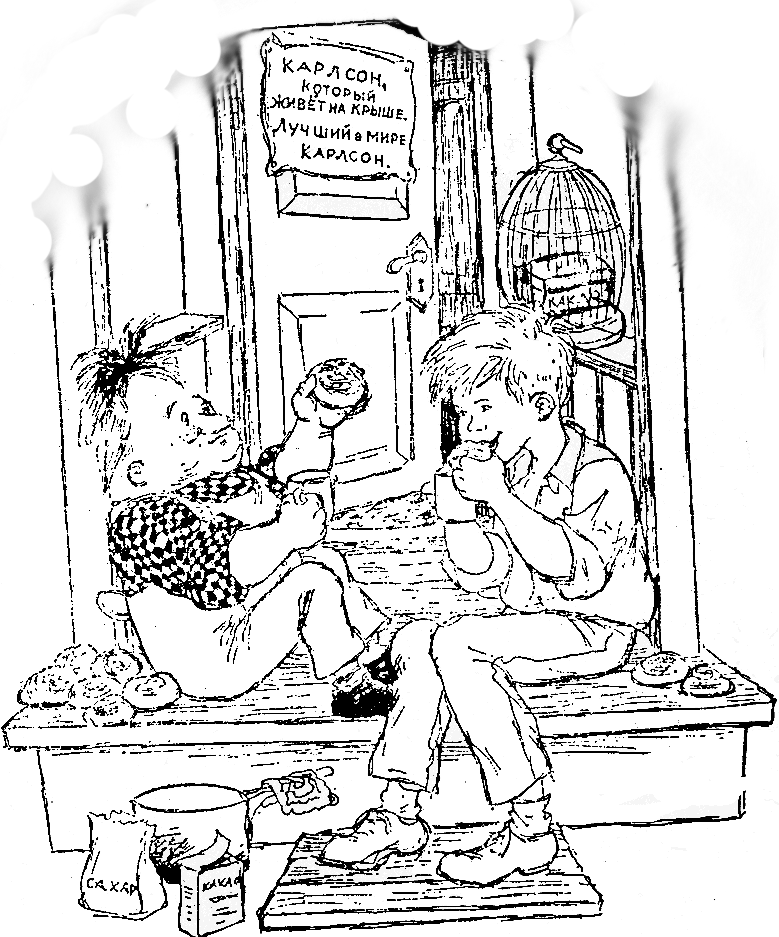
\includegraphics[scale=0.17]{./img/karlson}\hfill~
\end{minipage}
\begin{minipage}{0.55\linewidth}
\epigraph{
\textit{- Мы поделим их поровну: $7$ тебе и $7$ мне, - сказал Карлсон.\\
- Но так не получится, - возразил Малыш. -\\  $7+7=14$, а у нас только $10$ плюшек.\\
- В нынешних школах как-то по-дурацки считают, - ответил тот. - но я из-за этого страдать не намерен. По крайней мере, свои я уже взял, - добавил он и прикрыл пухлой ладошкой дымящуюся горку.
}}{Астрид Линдгрен «Три повести о Малыше и Карлсоне».}
\end{minipage}
\end{figure}

По определению целое число $а$ делится на не равное нулю целое число $b$, если существует целое число $q$ такое, что $a = bq$. В этом случае число $a$ называется делимым, $b$ - делителем, а $q$ - частным. В дальнейшем, речь будет идти только о целых числах.

\fbox{\begin{minipage}{0.95\textwidth}
\begin{ex}\label{u22}
	Запишите общий вид чисел, делящихся а) на 2; б) на 17; в) на 2012.
\end{ex}
\end{minipage}}

\begin{floatingfigure}[r]{0.2\textwidth}\setlength{\parindent}{0em}
	
\includegraphics[scale=0.35]{./img/dog}
\end{floatingfigure}
В литературе существует несколько способов обозначить делимость:

Если целое число $a$ делится на целое число $b$, то говорят, что $a$ кратно $b$, пишут $a\del b$. Соответственно запись $a\ndel b$ означает, что $a$ не делится на $b$, или $a$ не кратно $b$. 


Наряду с такими обозначениями используются запись $b~|~a$, означающая, что $a$ делит $b$, т.е. $a$ является делителем $b$. Запись $b~\mathrlap{\backslash}|~a$, что означает, что $a$ не делит $b$, т.е. $a$ не является делителем $b$.


Делимость целых чисел обладает несколькими основными свойствами:

\fbox{\begin{minipage}{0.95\textwidth}
\begin{prop}\label{pr1}
Если $a$ и $b$ делятся на $c$, то их сумма и произведение тоже делятся на $c$.
\end{prop}
\end{minipage}}

\begin{dok}
    Поскольку $a\del c$ и $b\del c$, то $a = cq_1$ и $b = cq_2$, где $q_1$ и $q_2$ - целые числа. Следовательно,  $a + b = c(q_1 + q_2)$ и $ab = c_2(q_1q_2)$. Что означает по определению, что $(a + b) \del c$ и $(ab) \del c$, поскольку если    $q_1$ и $q_2$ - целые числа, то их сумма и произведение также являются целыми числами. 
\end{dok}

\fbox{\begin{minipage}{0.95\textwidth}
\begin{prop}\label{pr2}
Если $a\del c$, но $b\ndel c$, то $(ab)\del c$, и $(a + b)\ndel c$.
\end{prop}
\end{minipage}}

\begin{dok}
1) Поскольку $a\del c$, то $a = cq$, где $q$ - целое число. Следовательно, $ab = c(qb)$, т.е. $(ab)\del c$.

2) Доказательство того, что $(a + b)\ndel c$, будем проводить методом «\textit{от противного}». Предположим, что $(a + b)\del c$, тогда из доказанного выше свойства следует, что $(a + b) + (-a)\del c$,\footnote{Здесь одно из слагаемых равно $(a + b)$ , а другое $(-a)$. Вообще говоря, здесь в неявном виде используется утверждение, что «если $a$ делится на $с$, то и $(-a)$ делится на $с$». Докажите это утверждение самостоятельно!} т.е. $b\del c$, но $b \ndel c$ по условию, значит мы пришли к противоречию. Итак, наше предположение, что $(a + b)\del c$, было неверно,  следовательно, $(a + b) \ndel c$.\footnote{При доказательстве теоремы методом «\textit{от противного}» сначала допускают, что утверждение этой теоремы неверно. Затем посредством некоторых рассуждений стараются получить либо заведомо неверное утверждение, либо утверждение, противоречащее условию теоремы. При правильных рассуждениях противоречие может получиться только за счет того, что неверным было первоначальное допущение о том, что теорема неверна. Отсюда делают вывод, утверждение теоремы верно.}
\end{dok}

Пользуясь основными свойствами, решите следующие задачи:

\begin{thm}\label{4.1}
	Докажите, что, если $a\del b$, и $b\del c$, то $a\del c$.
\end{thm}

\begin{thm}\label{4.2}
	Пусть $a \del c$, и $b \del d$. Докажите, что $(ab) \del (cd)$.
\end{thm}

\begin{thm}\label{4.3}
	Даны два числа $a$ и $b$ такие, что $a\del b$. Можно ли утверждать, что $a^n\del b^n$ при любом натуральном $n$?
\end{thm}

\begin{prim}
    Эти задачи входят в листок по теории чисел уровня 1.
\end{prim}

\fbox{\begin{minipage}{0.95\textwidth}

\begin{ex}\label{u23}
	Запишите условия предыдущих задач и свойств, используя вместо символа $\del$ символ $|$ .
\end{ex}
\end{minipage}}

\section{Деление с остатком.}

\epigraph{
\textit{Действительность никогда не делится на разум без остатка.
}}{Автор неизвестен}

Отметим на числовой оси точки, соответствующие целым числам. Пусть $b$ - некоторое натуральное (целое положительное) число. Выделим на рисунке все целые числа, кратные $b$. Они расположены на оси на равном расстоянии $b$ друг от друга (Рис. \ref{axis1}). Каждое из этих чисел имеет общий вид $bt$, где $t$ - некоторое целое число. 

\begin{figure}[h]
\begin{subfigure}{.5\textwidth}
  \centering
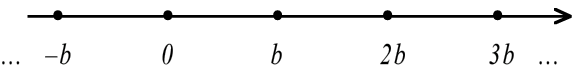
\includegraphics[width=.8\linewidth]{./img/axis1}
  \caption{}
  \label{axis1}
\end{subfigure}%
\begin{subfigure}{.5\textwidth}
  \centering
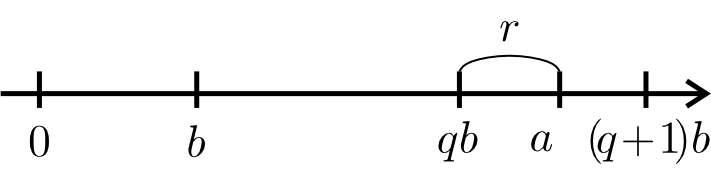
\includegraphics[width=.8\linewidth]{./img/axis2}
  \caption{}
  \label{axis2}
\end{subfigure}
  \caption{}
\end{figure}

Как было определено в начальной школе, если $a = qb$, то $q$ - это частное от деления $a$ на $b$. Будем считать, что остаток в данном случае равен $0$. Попробуем ввести понятие остатка, если целое число $a$ не делится на $b$. Раз $a$ не кратно $b$, то оно попадает между двумя выделенными числами, пусть эти числа $qb$ и $(q+1)b$ (Рис. \ref{axis2}). Тогда число $r = a - qb$ есть целое число, удовлетворяющее неравенству $0 < r < b$. В этом случае назовем частным число $q$, а остатком число $r$. 

Теперь сформулируем общее утверждение:

\fbox{\begin{minipage}{0.95\textwidth}
Если $a$ и $b$ - целые числа, причем $b$ больше нуля, то существуют такие целые числа $q$ и $r$, что $a = bq + r$, где $r$ удовлетворяет неравенству $0  \leqslant r < b$. Эти числа $q$ и $r$ определяются по данным $a$ и $b$ единственным образом. Частным называется число $q$, а остатком число $r$.
\end{minipage}}

Чтобы найти частное $q$ и остаток $r$, не нужно, конечно, рисовать отрезок длины $a$ на числовой оси и «укладывать» на нем много раз отрезок длины $b$. Для этого существует более рациональный способ. Это - известное всем правило деления одного числа a на другое число $b$ «столбиком». Это деление можно производить до тех пор, пока остаток не станет меньше, чем делитель. Например, если делить 1999 на 17, то при делении получается частное 117 и остаток 10.

\begin{prim}
В утверждении, обведенном в рамочку, сказано, что делитель $b$ - положительное число, и остаток таков, что $0  \leqslant r < b$, но делимое $a$ при этом может быть как положительное, так и отрицательное или вообще равное $0$. Например, $a = -22$, $b = 7$, тогда   $(-22) = (-4)\cdot 7 + 6$, где $0 \leqslant 6 <7$, т.е. остаток при делении $(-22)$ на 7 равен 6.
\end{prim}

\fbox{\begin{minipage}{0.95\textwidth}
\begin{ex}\label{u24}
	Какой остаток дает число\\
а) -1 при делении на 7;\hfillб) (-150) при делении на 19;\hfillв) (-54321) при делении на 4?
\end{ex}
\begin{ex}\label{u25}
	Докажите, что числа а) $10^4$ и $10^6$; \hfill    б) $10^5$ и $-1$;    \hfill   в) -123456789 и 9876543210 	\\
дают одинаковые остатки при делении на 11.
\end{ex}
\end{minipage}}

\newpage
Докажем основные свойства остатков:

\fbox{\begin{minipage}{0.95\textwidth}
\begin{prop}
Если к произвольному целому числу $x$ прибавить число $y$, делящееся на $c$, то остаток при делении $x$ на $c$ не изменится.
\end{prop}
\end{minipage}}

\begin{dok}
Пусть $x = cq + r$, $y  = cs$, тогда $x$ будет равен $c(q + s) + r$, где $0 \leqslant r < c$,\footnote{Объясните, почему это неравенство верно.} т.е. остаток не изменился.
\end{dok}

\fbox{\begin{minipage}{0.95\textwidth}
\begin{prop}
Если при делении на $c$ целые числа $a$ и $b$ дают остатки $r_1$ и $r_2$ соответственно, тогда суммы      $(a + b)$ и $(r_1 + r_2)$ при делении на $c$ дают одинаковые остатки.
\end{prop}
\end{minipage}}

\begin{dok}
Пусть $a = cq_1 + r_1$, $b = cq_2 + r_2$, тогда $(r_1 + r_2) = (a + b) - c(q_1 + q_2)$. Из доказанного выше свойства $0$ следует, что $(a + b)$ и $(r_1 + r_2)$ при делении на $c$ дают одинаковые остатки. 
\end{dok}

\fbox{\begin{minipage}{0.95\textwidth}
\begin{prop}
Если при делении на $c$ целые числа $a$ и $b$ дают остатки $r_1$ и $r_2$, тогда произведения $(ab)$ и $(r_1r_2)$ при делении на $c$ дают одинаковые остатки.
\end{prop}
\end{minipage}}

\begin{dok}
Пусть $a = cq_1 + r_1$, $b = cq_2 + r_2$, тогда $(r_1r_2) = (ab) - c(q_1q_2с + q_1r_2 + r_1q_2)$, т.е. $(ab)$ и $(r_1r_2)$ при делении на $c$ дают одинаковые остатки, т.к. отличаются на число, кратное $c$.
\end{dok}

С помощью этих свойств очень легко находить остатки.\footnote{По существу мы с вами доказали, что если нам интересуют только остатки, то на любом шаге вычислений мы можем рассматривать только остатки, пренебрегая целой частью.}

\begin{samp}
16131 при делении на 13 дает остаток 2. Действительно,   $16131 = 131 + 16\cdot10\cdot10$,    где 131 дает остаток 1,  а у числа $16\cdot10\cdot10$ такой же остаток, как и у числа  $3\cdot(-3)\cdot(-3)$. Остаток у 16131 такой же, как остаток у числа $(1+27)$, значит, он равен 2.
\end{samp}

Рассмотрим все числа, которые дают остаток $r$ при делении на $b$. Чтобы отметить все такие числа на числовой оси, надо взять отмеченные ранее числа, кратные $b$ (Рис. \ref{axis1}), и сдвинуть их вправо на $r$ (Рис. \ref{axis3})

\begin{figure}[h]
  \centering
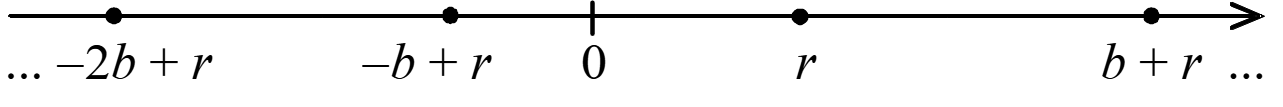
\includegraphics[width=.5\linewidth]{./img/axis3}
  \caption{}
  \label{axis3}
\end{figure}

Отметим, что общий вид числа, дающего остаток $r$ при делении на $b$, это $x = bt + r$,\footnote{Заметим, что в качестве $r$ вовсе не обязательно брать остаток от деления, можно взять любое другое число, дающее тот же остаток. Просто взятие остатка зачастую является наиболее удобным для понимания того, как устроен данный набор чисел.} где $t$ - произвольное целое число. Пусть в этой формуле $t$ пробегает все множество чисел {..., 2, 1, 0, 1, 2,...}, в то время как $b$ и $r$ фиксированы и не меняются (скажем, $b=8$,  $r=5$, тогда $x=8t+5$). При этом формула дает все возможные целые числа, для которых остаток от деления на $b$ равен $r$. Если изобразить эти числа на оси, то получится множество точек, отстоящих друг от друга на расстоянии $b$ (см. Рис. \ref{axis3} и Рис. \ref{axis4} - на последнем приведено множество точек $x=8t+5$).

\begin{figure}[h]
  \centering
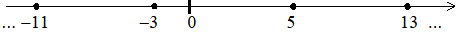
\includegraphics[width=.5\linewidth]{./img/axis4}
  \caption{}
  \label{axis4}
\end{figure}

Таким образом, если задано $b > 0$, то все множество целых чисел можно разбить на $b$ классов: к одному классу отнести все числа, дающие при делении на $b$ остаток 1, к другому - остаток 2, и так далее. Эти классы можно записать так:

\begin{center}
    $x=bt+1$; \hspace{3mm} $x=bt+2$; \hspace{3mm} ...; \hspace{3mm} $x=bt+(b-1)$
\end{center} 

и, наконец, последний (вернее «нулевой») класс $x = bt$. В него входят все числа, дающие при делении на $b$ остаток 0, т.е. делящиеся на $b$. (Например, если $b=8$, то всего классов 8: $x = 8t$, $x = 8t + 1,$ ..., $x = 8t + 7$.) Каждое число обязательно попадает в один и только в один класс. То есть число не может давать двух различных остатков при делении на одно и то же число.\footnote{Это утверждение означает корректность определения деления с остатком.}

\newpage

ИТАК:

Множество всех чисел $с$ остатком $r$ при делении на $b$ образуют один класс, называемый классом $r$ по модулю $b$ (например, класс 5 по модулю 8 это множество всех чисел, которые дают остаток 5 при делении на 8). Если взять произвольное целое число $x$ и рассмотреть его по модулю $n$, то чтобы определить в каком классе находится наше число, надо рассмотреть его остаток при делении на $n$ (например, $x = 13$, а $n = 8$, тогда число $x$ попадает в класс 5 по модулю 8). Таким образом, если взять натуральное число $n$, то все целые числа разбиваются ровно на $n$ классов, и каждое целое число попадает ровно в один из них.\footnote{Заметим, что множества всех целых чисел, дающих одинаковый остаток при делении на $n$, называют также классами вычетов по модулю $n$. Обозначают $ \tilde{d} = \{ z \in \mathbb{Z} | z - d \del n\}$ - это все числа, имеющие одинаковый с числом $d$ остаток при делении на $n$. Например, числа -1, 3, 7 попадают в класс вычетов $\tilde{3}$ по модулю 4.}

\underline{Обозначение}: A $\equiv$ B (mod C), если А и В дают одинаковые остатки при делении на С.

\fbox{\begin{minipage}{0.95\textwidth}
\begin{ex}\label{u26}
	Запишите общий вид числа, которое при делении а) на 22 дает такой же остаток, что и 2012; б)  на 13 дает такой же остаток, что и 31; в) на 2012 дает такой же остаток, что и (-22).
\end{ex}
\begin{ex}\label{u27}
    Определите, к какому классу относится число а) 2012 по модулю 17; б) 2012 по модулю 2011; в) (-2010) по модулю 22; г) $2004^{13}$ по модулю 1024?
\end{ex}
\begin{ex}\label{u28}
    Выясните, какие из утверждений являются верными: \\
    а) 5 $\equiv$ 17 (mod 2); б) 21 $\equiv$ 154 (mod 5); в) -21 $\equiv$ 154 (mod 5); г) 2007 $\equiv$ 2021 (mod 19); д) 1234567897 $\equiv$ 7987654321 (mod 9); е) 17 $\equiv$ -17 (mod 3).
\end{ex}
\begin{ex}\label{u29}
    Может ли целое число одновременно находиться в классах 1 по модулю 7, 1 по модулю 9, 1 по модулю 11, 1 по модулю 13? (Если да, то приведите пример такого числа, если нет, то докажите, что их нет.) 
\end{ex}
\end{minipage}}

\fbox{\begin{minipage}{0.95\textwidth}
\begin{prop}
Два числа $x_{1}$ и $x_{2}$ попадают в один и тот же класс по модулю $b$ в том и только в том случае, если их разность $x_1 - x_2$ делится на $b$. 
\end{prop}
\end{minipage}}

Выше мы уже говорили, что числа, делящиеся на $n$, расположены на числовой оси «равномерно», то есть через каждые $n$ - 1 чисел. Как каждое второе число является четным (и, соответственно, среди двух последовательных чисел обязательно найдется четное) так и каждое третье число делится на 3 (и, соответственно, среди трех последовательных чисел будет ровно одно, делящееся на три). Эти свойства используются при решении многих задач.

\begin{thm}\label{4.4}
	Докажите, что произведение трех последовательных чисел делится на 6.
\end{thm}

\begin{dok}
    Поскольку среди любых двух последовательных чисел одно обязательно четное, то произведение делится на 2. Кроме того, среди любых трех последовательных чисел одно обязательно делится на 3, значит, произведение делится на 3. Поэтому произведение делится на 6. 
\end{dok}
\begin{floatingfigure}[L]{0\textwidth}
\end{floatingfigure}

\textit{\textbf{Внимание!}} Мы при доказательстве воспользовались тем фактом, что если число (в данном случае произведение трех последовательных чисел) делится на 2 и на 3, то оно делится на 6. Более общий факт: 

\fbox{\begin{minipage}{0.95\textwidth}
\begin{prop} 
Если число А делится на $b$ и делится на $с$ и числа $b$ и $с$ взаимно просты (то есть не имеют общих делителей), то А делится на произведение $bс$. 
\end{prop}
\end{minipage}}

\begin{thm} 
	Докажите, что при любом натуральном $n$ число $n^3 - n$ кратно 6.
\end{thm}

\begin{dok}
    $n^3 - n  =  (n - 1) n (n + 1)$ - произведение трех последовательных чисел. Как было доказано в задаче \ref{4.4}, оно делится на 6.
\end{dok}
\begin{floatingfigure}[L]{0\textwidth}
\end{floatingfigure}

\newpage

\begin{center}
	{\large\textbf{Десятичная запись числа}}
\end{center}

\epigraph{\textit{Многие думают, что деньги - это бактерии, которые размножаются делением. Правда, так они думают только о чужих деньгах, а свои деньги просто обязаны размножаться умножением.}}{Из заметок в Интернете}

У чисел, с которыми мы работаем, есть единицы, десятки, сотни… Часто, когда точно неизвестно, каково количество этих самых единиц, десятков, сотен, используют запись с неизвестными: $\overline{xyz}$ - это число, в котором $x$ сотен, $y$ десятков и $z$ единиц, т.е. $\overline{xyz} = 100x + 10y + z$ . В следующих двух  задачах будет полезно представлять числа именно в таком виде. 

\fbox{\begin{minipage}{0.95\textwidth}
\begin{ex}\label{u30}
	Что за числа зашифрованы в записи: а) $\overline{1x}$; б) $\overline{xy5}$; в) $\overline{ab1c0}$ ?
\end{ex}
\begin{ex}\label{u31}
    Пусть некоторое число $a$ делится на простое число $p$. Что вы можете сказать про $a^2$? а про $a^n$?
\end{ex}
\begin{ex}\label{u32}
    Пусть A - квадрат некоторого числа. Выясните, на какую цифру может заканчиваться A?
\end{ex}
\begin{ex}\label{u33}
     Известно, что A = $x^2$. При этом A делится на 3. Что вы можете сказать про число $x$?
\end{ex}
\begin{ex}\label{u34}
    Известно, что A = $x^2$. При этом A делится на 2007. Что вы можете сказать про число $x$?
\end{ex}
\end{minipage}}

\section{Ответы к упражнениям}
\textbf{\ref{u22}.} а)~$2n$, где $n$ - целое; б)~$17n$, где $n$ - целое; в)~$2012n$, где $n$ - целое. 
\textbf{\ref{u23}.} \textbf{Свойство \ref{pr1}}:~если $c~|~a$  и $c~|~b$, то $c~|~(a~+~b)$ и $c~|~(ab)$; \textbf{Свойство \ref{pr2}}:~если $c~|~a$, но $c~\mathrlap{\backslash}|~b$, то $с~|~ab$, но $c~\mathrlap{\backslash}|~(a+b)$; \textbf{Задача \ref{4.1}}:~докажите, что, если $c~|~b$, а $b~|~a$, то $c~|~a$; \textbf{Задача \ref{4.2}}:~пусть $c~|~a$, а $d~|~b$. Докажите, что $(cd)|(ab)$; \textbf{Задача \ref{4.3}}:~даны два числа $a$ и $b$ такие, что $b~|~a$. Можно ли утверждать, что $bn~|~an$ при любом натуральном $n$? 
\textbf{\ref{u24}.} а)~6; б)~2; в)~3.
\textbf{\ref{u26}.} а)~$22t+2012$ или $22t+10$; б)~$13t+31$ или $13t+5$; в)~$2012t-22$ или $2012t+1990$.
\textbf{\ref{u27}.} а)~$\tilde{6}$; б)~$\tilde{1}$; в)~$\tilde{14}$; г)~$\tilde{0}$.
\textbf{\ref{u28}.} а), в), д).
\textbf{\ref{u30}.} а)~число вида $10+x$, где $x$ - цифра; б)~число вида $100x+10y+5$; в)~число вида $10000a + 1000b + 100 + 10c$.
\textbf{\ref{u31}.} Тогда $a^2$ делится на $p^2$, а $a^n$ делится на $p^n$. 
\textbf{\ref{u32}.} На 0, 1, 4, 5, 6 или 9. 
\textbf{\ref{u33}.} Тогда $x$ также делится на 3.
\textbf{\ref{u34}.} $2007 = 9 \times 223$. Тогда $x$ обязательно делится на $3 \times 223 = 669$.